\subsection*{الف}

در این درخت، راس اول نمایانگر انتخاب اولیه عدد 
$\alpha$
است که می‌تواند یا ۱ یا -۱ باشد. 


سپس بازیکن اول (بازیکن 
$x$
) می‌تواند از میان ۱، ۲ یا ۴ انتخاب کند. 


بعد از انتخاب بازیکن اول، بازیکن دوم (بازیکن
$y$
) همچنین می‌تواند از میان ۱، ۲ یا ۴ انتخاب کند.

\begin{center}
	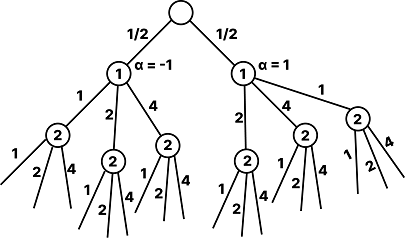
\includegraphics{tree}
\end{center}

راس‌های شامل عدد ۲ اطلاعات یکسان دارند.

\subsection*{ب}

برای یافتن استراتژی بهینه، باید با توجه به تابع سودی هر بازیکن به تحلیل بازی بپردازیم. این یک بازی صفر جمعی است، به این معنی که سود یک بازیکن به اندازه‌ی زیان بازیکن دیگر است. تابع سودی بازیکنان به شکل زیر است:


$$
u_1 = axy , u_2 = - axy
$$

هدف بازیکن اول افزایش
$u_1$ 
و هدف بازیکن دوم کاهش
$u_1$ 
(یا به عبارت دیگر، افزایش
$u_2$
) است.

با توجه به اینکه بازیکنان هر دو می‌توانند از بین اعداد ۱، ۲، و ۴ انتخاب کنند و مقدار a می‌تواند ۱ یا ۱- باشد، انتخاب بهینه برای هر دو بازیکن به شکل زیر است:

بازیکن اول (x) : با توجه به اینکه می‌خواهد
$u_1$ 
را افزایش دهد، باید x را برابر بزرگ‌ترین مقدار ممکن، یعنی ۴، قرار دهد.

بازیکن دوم (y) : با توجه به اینکه می‌خواهد
$u_1$ 
را کاهش دهد (یا
$u_2$ 
را افزایش دهد)، باید y را برابر کوچک‌ترین مقدار ممکن، یعنی ۱، قرار دهد.

بنابراین، استراتژی بهینه برای بازیکن اول
$x=4$
در صورتی که
$\alpha =1$
و در غیر این صورت
۱ را بازی می‌کند،
و برای بازیکن دوم
$y=1$
است.

همچنین لازم به ذکر است که در این تحلیل فرض کردیم که بازیکنان بهینه عمل می‌کنند و از اطلاعات موجود بهترین استفاده را می‌برند. در واقعیت، بازیکنان ممکن است به دلایل مختلف از این استراتژی‌های بهینه منحرف شوند.







